% \documentclass[UTF8,12pt]{article} % 12pt 为字号大小
\documentclass[12pt]{article}
\usepackage[utf8]{inputenc}
\usepackage{amssymb,amsfonts,amsmath,amsthm}
\usepackage{cite}
%\usepackage{fontspec,xltxtra,xunicode}
%\usepackage{times}

%----------
% 定义中文环境
%----------

\usepackage{xeCJK}

\setCJKmainfont[BoldFont={Heiti SC Light},ItalicFont={Kaiti SC Regular}]{Songti SC Regular}
\setCJKsansfont{Heiti SC Light}
\setCJKfamilyfont{song}{Songti SC Regular}
\setCJKfamilyfont{zhhei}{Heiti SC Light}
\setCJKfamilyfont{zhkai}{Kaiti SC Regular}
\setCJKfamilyfont{zhfs}{STFangsong}
\setCJKfamilyfont{zhli}{Libian SC Regular}
\setCJKfamilyfont{zhyou}{Yuanti SC Regular}

\newcommand*{\songti}{\CJKfamily{zhsong}} % 宋体
\newcommand*{\heiti}{\CJKfamily{zhhei}}   % 黑体
\newcommand*{\kaiti}{\CJKfamily{zhkai}}  % 楷体
\newcommand*{\fangsong}{\CJKfamily{zhfs}} % 仿宋
\newcommand*{\lishu}{\CJKfamily{zhli}}    % 隶书
\newcommand*{\yuanti}{\CJKfamily{zhyou}} % 圆体

%----------
% 版面设置
%----------
%首段缩进
\usepackage{indentfirst}
\setlength{\parindent}{2em}

%行距
\renewcommand{\baselinestretch}{1.4} % 1.4倍行距

%页边距
\usepackage[a4paper]{geometry}
\geometry{verbose,
  tmargin=2cm,% 上边距
  bmargin=2cm,% 下边距
  lmargin=3cm,% 左边距
  rmargin=3cm % 右边距
}


%----------
% 其他宏包
%----------
%图形相关
\usepackage[x11names]{xcolor} % must before tikz, x11names defines RoyalBlue3
\usepackage{graphicx}
\usepackage{pstricks,pst-plot,pst-eps}
\usepackage{subfig}
\def\pgfsysdriver{pgfsys-dvipdfmx.def} % put before tikz
\usepackage{tikz}
\usepackage{float}

%链接相关
\usepackage[colorlinks,linkcolor=black,anchorcolor=blue,citecolor=green]{hyperref}

%原文照排
\usepackage{verbatim}

%网址
\usepackage{url}

%算法相关
\usepackage{algorithm}
\usepackage{algorithmicx}
\usepackage{algpseudocode}

\floatname{algorithm}{算法}
\renewcommand{\algorithmicrequire}{\textbf{输入:}}
\renewcommand{\algorithmicensure}{\textbf{输出:}}

%----------
% 习题与解答环境
%----------
%习题环境
\theoremstyle{definition} 
\newtheorem{exs}{习题}

%解答环境
\ifx\proof\undefined\
\newenvironment{proof}[1][\protect\proofname]{\par
\normalfont\topsep6\p@\@plus6\p@\relax
\trivlist
\itemindent\parindent
\item[\hskip\labelsep
\scshape
#1]\ignorespaces
}{%
\endtrivlist\@endpefalse
}
\fi

\renewcommand{\proofname}{\it{证明}}


%==========
% 正文部分
%==========

\begin{document}

\title{平时作业1}
\author{1160300314 朱明彦}
\date{\today} % 若不需要自动插入日期,则去掉前面的注释;{ } 中也可以自定义日期格式
\maketitle

\section{作业要求}
在第一步中,如果初始化$U$、$V$矩阵的元素为一个相同的数,那么这个数设置多少,可以最小化例子矩阵的RMSE?

\begin{figure}[H]
  \centering
  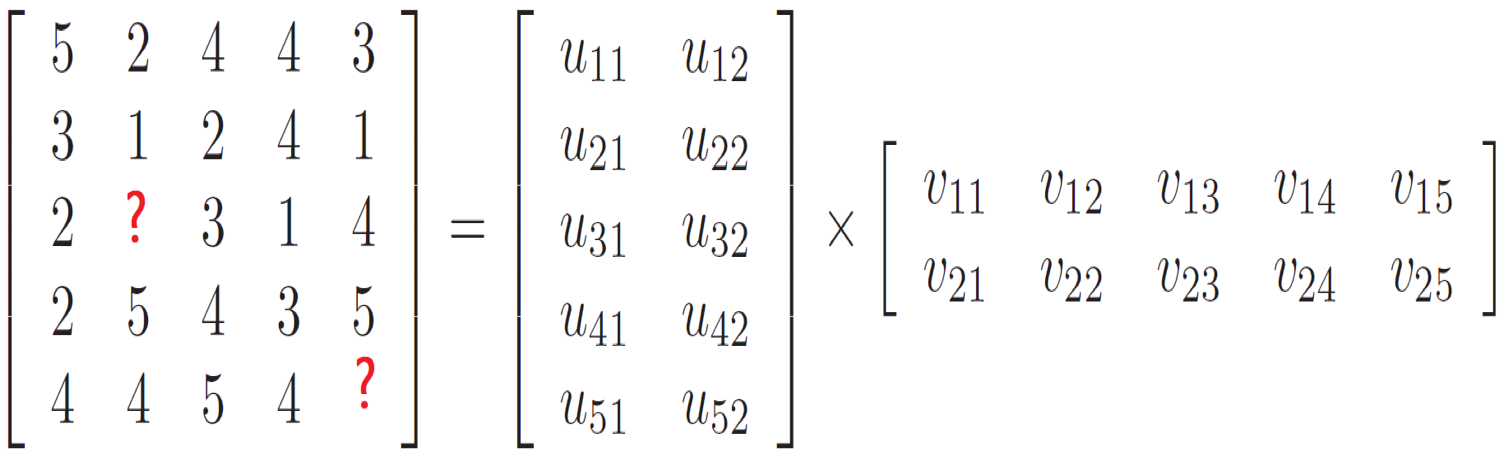
\includegraphics[width=0.8\linewidth]{fig/demand.png}
  \caption{作业要求}
  \label{fig:demand}
\end{figure}

\section{作业解答}
设原始矩阵为$M$, 分解后的矩阵为$U, V$, 则RMSE的计算公式如下:
$$
RMSE(M, U, V) = \sum_{i}^{n}\sum_{j}^{m}\sum_{M_{ij} \neq 0}\left(M_{ij} - \sum_{k}^{d}\left(U_{ik} \times V_{kj}\right)\right)^{2}
$$
由于$U, V$均被初始化为同一值, 所以设其为$x$, 又有$d = 2$, 可以有
$$
RMSE(M, U, V) = \sum_{i}^{n}\sum_{j}^{m}\sum_{M_{ij} \neq 0}\left(M_{ij} - 2x^2\right)^{2}
$$
为了计算的简便, 设$y = 2x^2$, 则有
$$
RMSE(M, U, V) = \sum_{i}^{n}\sum_{j}^{m}\sum_{M_{ij} \neq 0}\left(M_{ij} - y\right)^{2}
$$
对$RMSE$求导有
$$
\dfrac{\mathrm{d} RMSE }{\mathrm{d} y} = \sum_{i}^{n}\sum_{j}^{m}\sum_{M_{ij} \neq 0}\left(2y - 2M_{ij}\right)
$$
令$\frac{\mathrm{d} RMSE }{\mathrm{d} y} = 0$,将原始矩阵中的值带入后有
$$
y = \frac{75}{23}
$$
从而
$$
x = \pm \sqrt{\frac{75}{46}}
$$
所以当$x = \pm \sqrt{\frac{75}{46}}$时, RMSE取最小值.
\end{document}